\documentclass[a4paper,12pt]{article}
\usepackage[utf8]{inputenc}
\usepackage[T1]{fontenc}
\usepackage{geometry}
\usepackage{graphicx}
\usepackage{booktabs}
\usepackage{amsmath}
\usepackage{cite}
\usepackage{hyperref}
\usepackage{tocloft}
\usepackage{setspace}
\usepackage{float}

\usepackage{tikz}
\usetikzlibrary{arrows.meta, positioning}
\tikzset{
	gene/.style={circle, draw, minimum size=8mm, font=\sffamily},
	activate/.style={-{Stealth[length=3mm]}, thick},
	activate dashed/.style={-{Stealth[length=3mm]}, thick, dashed},
	suppress/.style={-|, thick}
}


\geometry{margin=1in}
\onehalfspacing


\renewcommand{\cftsecleader}{\cftdotfill{\cftdotsep}}

\title{Project Report: [Dynamical analyze of GRN for AML]}
\author{[ Yasaman Safayi Konjin \\ Spehr Salmani Yeganeh \\ Sara Akbari Khorram] \\ [physics , sharif university of technology] \\ [Your Email(s)]}
\date{September 2025}

\begin{document}

\begin{titlepage}
	\centering
	{\large Sharif University of Technology\par}
	\begin{figure}
		\centering
		
\includegraphics[width=0.5\linewidth]{csm_kisspng-sharif-university-of-technology-university-of-teheran_7c97300984.png}
		\label{fig:placeholder}
	\end{figure}
	{\large Physics Department \\ Special Topics in Statistical Physics \par}
	\vspace{1 cm}
	{\Huge \bfseries Dynamical Analyze of GRN for AML \par}
	\vspace{1cm}
	{\Large Yasaman Safayi Konjin \\ Sepehr Salmani Yeganeh \\ Sara Akbari Khorram \par}
	\vspace{1 cm}
	
	{\large spring of 2025 \par}
\end{titlepage}

\clearpage

\tableofcontents
\clearpage


%%%%%%%%%%%%%%%%%%%%%%%%%%%%%%%%%%%%%%%%%%%%%%%%%%%%%%%%%%%%%%%%%%%%%%%%%%%
%%%%%%%%%%%%%%%%%%%%%%%%%%%%%%%%%%%%%%%%%%%%%%%%%%%%%%%%%%%%%%%%%%%%%%%%%%%
\section*{Abstract}
\addcontentsline{toc}{section}{Abstract}
This report presents the outcomes of a collaborative project focused on analyzing the dynamics of the gene regulatory network (GRN) associated with acute myeloid leukemia (AML). The primary objective was to develop a computational model to reconstruct AML’s GRN, enabling the study of the disease through the activities of its most influential transcription factors.
Initially, comprehensive data on AML were collected from relevant literature to inform the modeling process. The innovative aspect of this project lies in analyzing network dynamics using a physics-based approach—specifically, leveraging the Jacobian matrix, a method not previously applied in this context.
A Python-based model was developed to generate a dataset capturing potential irregular dynamics that may contribute to cancer development. This dataset was analyzed using the k-means clustering method to identify patterns in transcription factor activity. The results demonstrated a promising alignment with documented transcription factor behaviors in AML cases reported in the literature.
Furthermore, a Random Forest machine learning algorithm was employed to detect irregularities in transcription factor activities and diagnose underlying dynamics. These findings offer valuable insights into AML’s genetic dynamics and pave the way for future research in targeted diagnostics and therapeutic strategies.


%%%%%%%%%%%%%%%%%%%%%%%%%%%%%%%%%%%%%%%%%%%%%%%%%%%%%%%%%%%%%%%%%%%%%%%%%%%
%%%%%%%%%%%%%%%%%%%%%%%%%%%%%%%%%%%%%%%%%%%%%%%%%%%%%%%%%%%%%%%%%%%%%%%%%%%
\section{Introduction}
\subsection{Problem Statement}
\textit{Acute Myeloid Leukemia} (AML) is a complex hematologic malignancy characterized by dysregulated gene expression, driven by aberrant dynamics in its \textit{gene regulatory network} (GRN). Despite advances in understanding AML’s molecular basis, current computational models often fail to capture the intricate dynamics of transcription factor interactions that drive disease progression. Traditional approaches to GRN analysis—such as differential expression studies—lack the capacity to model the nonlinear and dynamic behavior of gene interactions, limiting their effectiveness in identifying critical regulatory patterns.

Moreover, there remains a gap in applying physics-based methodologies, such as Jacobian matrix analysis, to the study of AML’s GRN - an approach that could uncover novel insights into its genetic dynamics. This project addresses the need for an innovative computational framework to reconstruct and analyze AML’s GRN, with a focus on identifying irregular transcription factor activities. By leveraging a physics-based approach, this study aims to deepen our understanding of AML’s regulatory mechanisms and support the development of targeted diagnostic and therapeutic strategies.

%%%%%%%%%%%%%%%%%%%%%%%%%%%%%%%%%%%%%%%%%%%%%%%%%%%%%%%%%%%%%%%%%%%%%%%%%%%
\subsection{Objectives}
The objectives of this project are as follows:
\begin{enumerate}
	\item To develop a computational model for reconstructing the gene regulatory network (GRN) of acute myeloid leukemia (AML) using a physics-based approach that leverages the Jacobian matrix.
	\item To generate a dataset that captures irregular dynamics in transcription factor activities potentially contributing to AML progression.
	\item To analyze the generated dataset using the k-means clustering method in order to identify patterns in transcription factor behavior.
	\item To implement a Random Forest machine learning algorithm for detecting and diagnosing irregularities in transcription factor activities within the AML GRN.
	\item To validate the model’s findings against existing literature, assessing its accuracy and potential to advance targeted diagnostic and therapeutic strategies.
\end{enumerate}



%%%%%%%%%%%%%%%%%%%%%%%%%%%%%%%%%%%%%%%%%%%%%%%%%%%%%%%%%%%%%%%%%%%%%%%%%%%
%%%%%%%%%%%%%%%%%%%%%%%%%%%%%%%%%%%%%%%%%%%%%%%%%%%%%%%%%%%%%%%%%%%%%%%%%%%
\section{Methodology}
\label{sec:methodology}
This section outlines the computational methods used to reconstruct and analyze the gene regulatory network (GRN) of acute myeloid leukemia (AML), focusing on the dynamics of six transcription factors: CEBPA, SPI1, MYB, RUNX1, HOXA9, and MEIS1.

\begin{figure}[H]
	\centering
	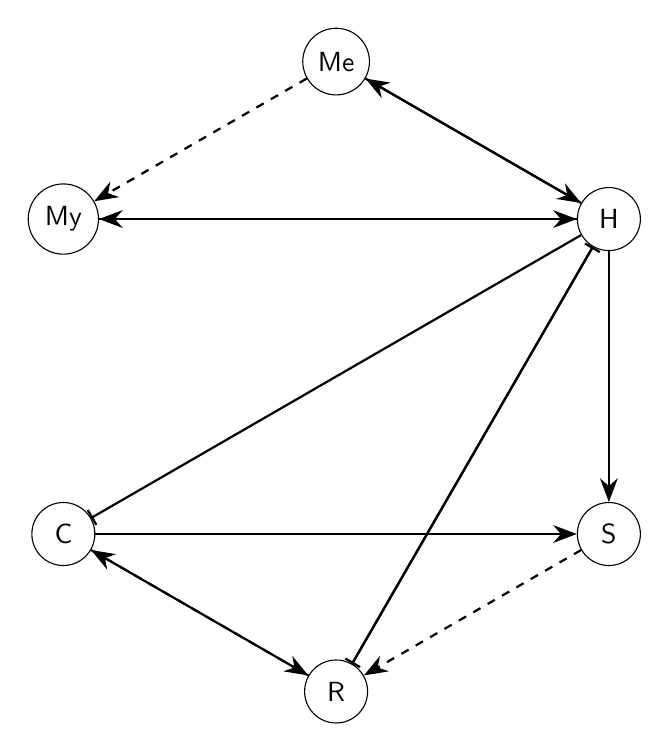
\begin{tikzpicture}[node distance=2cm]
		
		% Place nodes in a circle
		\node[gene] (Me) at (90:4cm) {Me};
		\node[gene] (H)  at (30:4cm) {H};
		\node[gene] (S)  at (-30:4cm) {S};
		\node[gene] (R)  at (-90:4cm) {R};
		\node[gene] (C)  at (-150:4cm) {C};
		\node[gene] (My) at (150:4cm) {My};
		
		% Edges
		\draw[activate dashed] (Me) -- (My);   % Me -> My (dashed)
		\draw[activate] (Me) -- (H);            % Me -> H (solid)
		
		\draw[activate dashed] (My) -- (H);     % My -> H (dashed)
		
		\draw[activate] (H) -- (My);            % H -> My (solid)
		\draw[activate] (H) -- (Me);            % H -> Me (solid)
		\draw[suppress] (H) -- (R);             % H -| R
		\draw[suppress] (H) -- (C);             % H -| C
		\draw[activate] (H) -- (S);             % H -> S
		
		\draw[activate] (C) -- (S);             % C -> S
		\draw[activate dashed] (C) -- (R);      % C -> R (dashed)
		
		\draw[activate dashed] (S) -- (R);      % S -> R (dashed)
		
		\draw[activate] (R) -- (C);             % R -> C
		\draw[suppress] (R) -- (H);             % R -| H
		
	\end{tikzpicture}
	\caption{Gene regulatory network showing activation (solid/dashed arrows) and suppression (flat-head lines) among Me, My, H, R, C, and S.}
	\label{fig:gene_network}
\end{figure}

%%%%%%%%%%%%%%%%%%%%%%%%%%%%%%%%%%%%%%%%%%%%%%%%%%%%%%%%%%%%%%%%%%%%%%%%%%%
\subsection{Data Collection and Parameter Setup}
\label{subsec:data_collection}
A simulated dataset was generated to represent the dynamics of AML’s GRN, focusing on six transcription factors. Interaction parameters were defined as a symbolic matrix \( A \) with 19 parameters (e.g., \( cc \), \( rc \), \( hc \)), representing regulatory interactions. Mean and standard deviation values for scaling fixed points were assigned based on hypothetical RNA-seq data.

%%%%%%%%%%%%%%%%%%%%%%%%%%%%%%%%%%%%%%%%%%%%%%%%%%%%%%%%%%%%%%%%%%%%%%%%%%%
\subsection{Model Development}
\label{subsec:model_development}
A Python-based computational model was developed to reconstruct AML’s GRN using the Jacobian matrix. The matrix \( \mathbf{A} \), representing GRN interactions, was constructed using \texttt{SymPy} for symbolic computations and converted to numerical form with \texttt{NumPy} and \texttt{SciPy}. The condition for non-zero fixed points was derived by solving \( \det(\mathbf{A}) = 0 \) for the parameter \( cc \).

To ensure a robust representation of the GRN and mitigate matrix sparsity, hypothetical regulatory links were incorporated into the symbolic matrix. A total of 42,208 valid parameter sets were generated by randomly sampling 18 parameters within predefined ranges (e.g., \( \texttt{activation constants} \in [0.01, 2] \), \( \texttt{suppression constants} \in [-2, -0.01] \), \( \texttt{self-activation and suppression rate} \in [-2, 2] \), \( \texttt{hypothetical links} \in [0, 1] \)), while ensuring \( \det(\mathbf{A}) \approx 0 \). Fixed points were computed using the null space of \( \mathbf{A} \) and scaled to RNA-seq ranges using predefined means and standard deviations. Data generation continued iteratively until exactly \( \texttt{number\_of\_stable\_fixed\_points} = 512 \) stable fixed points were obtained, ensuring sufficient representation of stable system dynamics for downstream analyses.


%%%%%%%%%%%%%%%%%%%%%%%%%%%%%%%%%%%%%%%%%%%%%%%%%%%%%%%%%%%%%%%%%%%%%%%%%%%
\subsection{Dynamic Analysis}
\label{subsec:dynamic_analysis}
The dynamics of the GRN were analyzed by computing the eigenvalues of the numerical Jacobian matrix \( \mathbf{A} \). The real parts of the eigenvalues were used to classify the system’s behavior into Stable, Unstable, Saddle, or Non-zero Fixed Point dynamics, with a threshold of \( \pm 0.0001 \). 

%%%%%%%%%%%%%%%%%%%%%%%%%%%%%%%%%%%%%%%%%%%%%%%%%%%%%%%%%%%%%%%%%%%%%%%%%%%
\subsection{Clustering Analysis}
\label{subsec:clustering}
The fixed points dataset, comprising expression levels of the six transcription factors, was normalized using \texttt{StandardScaler} from \texttt{scikit-learn}. The k-means clustering algorithm was applied to identify patterns in transcription factor dynamics, with the optimal number of clusters determined using the silhouette score over a range of \( k = 2 \) to 9. Clustering results were visualized in 2D and 3D using UMAP (\texttt{n\_neighbors=30}, \texttt{min\_dist=0.5}) and PCA, implemented with \texttt{umap-learn} and \texttt{scikit-learn} libraries, respectively. Visualizations were generated using \texttt{Matplotlib} and \texttt{Plotly} to analyze cluster distributions.

\subsection{Diagnostic Modeling with Random Forest}
\label{subsec:diagnostic_modeling}
A Random Forest classifier, implemented via \texttt{scikit-learn}, was trained to classify GRN dynamics (Stable, Unstable, Saddle, Non-zero Fixed Points) based on the dataset of fixed points and interaction parameters. The dataset was split into training (80\%) and testing (20\%) sets using a random seed of 42 for reproducibility. Features were normalized using \texttt{StandardScaler}, and the model was trained on the scaled training data. Model performance was evaluated using accuracy, precision, recall, and F1-score metrics, as reported in a classification report.

\subsection{Validation}
\label{subsec:validation}
The clustering and classification results were validated by analyzing the distribution of dynamics within each cluster and computing statistical measures, such as the mean and standard deviation of fixed points and interaction parameters. The silhouette score assessed clustering quality, while the Random Forest model’s classification report ensured robust detection of dynamics. Findings were compared with documented AML transcription factor behaviors to evaluate their biological relevance.


\clearpage
\section{Results}
\label{sec:results}
.

\subsection{Key Findings}
.


\clearpage
\section{Discussion}
.

\clearpage
\section{Conclusion}
\label{sec:conclusion}
.

\end{document}